\documentclass[11pt]{amsart}
\usepackage[english]{babel}
\usepackage[utf8x]{inputenc}
\usepackage[T1]{fontenc}
\usepackage[numbers, sort&compress]{natbib}
\usepackage[a4paper,%
      top=3cm,%
      bottom=2cm,%
      left=3cm,%
      right=3cm,%
      marginparwidth=1.75cm]{geometry}
\usepackage{amsmath, amsthm, amssymb, amsfonts, enumerate}
\usepackage{graphicx}
\usepackage[colorinlistoftodos]{todonotes}
\usepackage[colorlinks=true, allcolors=blue]{hyperref}
\usepackage{booktabs}
\usepackage{siunitx}
\usepackage{cleveref}
\usepackage[foot]{amsaddr}
\usepackage{float}
\usepackage[section]{placeins}
%
\usepackage{color}
\usepackage[]{algorithm,algcompatible,lipsum}
\usepackage[]{algpseudocode}
\usepackage{listings}
\usepackage{moreverb}
%
\newtheorem{theorem}{Theorem}[section]
\newtheorem{lemma}[theorem]{Lemma}
\newtheorem{proposition}[theorem]{Proposition}
\newtheorem{assumption}[theorem]{Assumption}
\theoremstyle{definition}
\newtheorem{remark}[theorem]{Remark}
\newtheorem{example}[theorem]{Example}
\newtheorem{definition}[theorem]{Definition}
%

\numberwithin{equation}{section}


\newcommand{\R}{\mathbb{R}}
\newcommand{\N}{\mathbb{N}}
\newcommand{\s}{\subseteq}
\newcommand{\e}{\varepsilon}
%
%
%
%%title
\makeatletter
\renewcommand{\Function}[2]{%
  \csname ALG@cmd@\ALG@L @Function\endcsname{#1}{#2}%
  \def\jayden@currentfunction{#1}%
}
\newcommand{\funclabel}[1]{%
  \@bsphack
  \protected@write\@auxout{}{%
    \string\newlabel{#1}{{\jayden@currentfunction}{\thepage}}%
  }%
  \@esphack
}
\makeatother
\title[%
	Optimal policies in a family of epidemic models%
	]{
	Existence, characterization and simulation of optimal policies in a family of epidemic 
  models
}
%
%
\author[S. D\'iaz-Infante]{Saul D\'iaz-Infante}
\email{\tt sdinfante@conacyt.mx} 
\author[F. Pe\~nu\~n\'{u}ri]{Francisco Pe\~n\'u\~nuri}
\email{\tt francisco.pa@correo.uady.mx}
\author[D. Gonz\'alez-S\'anchez]{David Gonz\'alez-S\'anchez}
\email{\tt dgonzalezsa@conacyt.mx}
%
\address[S. D\'iaz-Infante, D. Gonz\'alez-S\'anchez]{
  Departamento de Matem\'aticas, 
  CONACYT-Universidad de Sonora,
  Hermosillo, Sonora.
}
\address[F. Pe\~n\'u\~nuri]{%
  Departamento de Ingenier\'ia F\'isica,
  Universidad Autónoma de Yucat\'an, 
  M\'erida Yucat\'an
}
%
%
\keywords{%
  SIR, optimal control, epidemic models, 
  forward-backward-sweep method, Pontryagin maximum principle}
\subjclass[2010]{49K15, 49M05, 92D30}
%
\begin{document}
  \begin{abstract}
    We survey some theoretical results about a family of optimal 
    control problems that arise in epidemiology. We also implement the
    so-called forward-backward-sweep method in Python to find approximate
    optimal control policies via the Pontryagin maximum principle. 
    In addition, four specific models are described and simulated.
  \end{abstract}
\maketitle
%
  \section{Introduction}
  %
      By the end of the Middle Ages, smallpox cut down the 
population in centers of Europe and Asia\textemdash three of each ten dies by 
smallpox\textemdash perhaps that gives its alias, "speckled monster."  
Although experts understand the mechanism of transmission of this  "monster"
until the early 20  century, it represents the first documented disease
\citep[][]{bernoulli1760essai, bradley1971smallpox, Foppa2017} against which a
specific control intervention was available: the inoculation. This process
relies on put material from smallpox sores to healthy people. Usually scratching
material over the armor or inhaling it through the nose. People develop the
symptoms associated with smallpox---fever and a rash. However, the death rate
due to inoculation is considerably lower than natural smallpox.

  Then Bernoulli naturally sets a question like this: What happens if everybody
were inoculated? Here, we address the question: How to inoculated in optimal
way? Throughout the following lines we answer and illustrate the implications
of this question. 

  Optimal control theory is a way to answer the above question.  In the
mid-fifties, Pontryagin and Bellman propose generalizations of the calculus of
variations of broad applicability:  the maximum principle and the method of
dynamic programming. Now, these results sustain application in the
biological sciences, and, in particular, to the optimal control
of infectious diseases.

  The approach in this work relies on Pontryagin's Maximum
Principle \cite{Boltyanski1960} and follows the same methodology of
\citet{lenhart2007optimal}. Lenhart's work makes an accessible optimal control
device to describe common epidemic interventions like vaccination, treatment,
quarantine, isolation among others. Our intention in this work is illustrate
the mentioned strategies throughout recent literature and state result for
existence of control solution for a particular family of epidemic models.
Likewise we present  important regarding goals and issues that appear with the
relating theory and numerical approximations. We start by fixing our notation
and enunciate the core of the theory.














\input{Notation.tex}











  \section{The uncontrolled SIR model}
      Infectious diseases sculpt civilizations.  HIV/AIDS, Spanish influenza, and
Black Death are the most devastating pandemics in human history. They have
killed more than 100 million people. Therefore, understand the mechanism of
spread and control of diseases of this kind is wide essential.
In this line, the SIR structure is a convenient option to model its 
spreading. 

  The SIR model is a compartmental structure. Primarily, the model consists of 
three compartments: susceptible $S$, infected $I$, and recovered $R$, %that 
 and transitions functions between compartments.

  Practically, all the existing epidemic models are variants of this structure. 
The variants emerge to describe particular characteristics of a disease, 
mechanism of transmission, population dynamics, among others. 
To fix ideas, consider the classic model of 
\citet{Kermac}
\begin{equation}
  \begin{aligned}
    \frac{dS}{dt} & = - \kappa SI
      \\
    \frac{dI}{dt} & = \kappa SI - \lambda I
      \\
    \frac{dR}{dt} & = \lambda I,
  \end{aligned}
\end{equation}
here the transition from the susceptible $S$ to the infected class $I$ 
occur with constant rate $\kappa$, and from  the infected class $I$ to the 
recovered happens with rate $\lambda$.

In next sections, we provide the main ideas to control modifications of this 
base structure with optimal policies.
  \section{Control policies in epidemics}
    Here the main reference is the book of Lenhart 
\cite{Lenhart2002}.
\paragraph{Introduction.}
\paragraph{Comments about recent bibliography.}
\paragraph{What means a optimal control policy in this context?}
\paragraph{Usual control policies.}
\paragraph{The cost function and its interpretation in epidemic control models.}
    \subsection{Culling}
      Here we present the model reported in \cite*{Bolzoni2014} to describe a 
outbreak of bovine tuberculosis. The regarding uncontrolled model reads

\begin{equation}
	\begin{aligned}
  \min_{u(t)\in \mathcal{U}}
    &
    \int_0^T
      I(t) + P [u(t)]^{\theta}, \quad \theta \in \{1,2\},
      \quad P = B/A
  \\ \textrm{subject to:} &
  \\
    &\dfrac{dS}{dt} =
			r S 
			\left (
				1 - \dfrac{S+I}{K}
			\right)
			 - \beta SI - u(t) S
		\\
		&\dfrac{dI}{dt} =
			\beta SI - (\alpha + \mu + u(t)) I.
	\end{aligned}
\end{equation}
%

    \subsection{Vaccination}
        Here we consider a standard epidemic model to describe the dynamics of a 
disease. We use optimal control techniques to find a vaccination
schedule for the disease. Goal is to minimize the number of infectious 
persons and the overall cost of the vaccine during a fixed time period. 

  Here $S(t)$,$I(t)$,$R(t)$ respectively denote the number of susceptible 
infectious, and recovered (immune) individuals at time $t$. The model also 
consider a class that represent the number of exposed $E(t)$. 
Then the whole population $N$ is given by $N(t) = S(t) + E(t) + I(t) + R (t)$,
and obeys the last equation of model \eqref{eqn:epidemics_lenhart}.

The control $u(t)$ is a fraction of susceptible individual being 
vaccinated per unit of time. Since vaccination of the entire susceptible 
population is impractical, the model considers $0 \leq u(t) \leq 0.9$. 

Hence, the optimal control problem reads\em parameters in 
\Cref{tbl:epidemics_lenhart_des}.


\begin{equation} \label{eqn:epidemics_lenhart}
  \begin{aligned}
    \min_{u} & \int_{0}^{T} AI(t) + u^{2}(t) dt,
    \\
    \text{subject to}
    \\
      \dot{S}(t) &=
          bN(t) - dS(t) - cS(t)I(t) - u(t)S(t), \quad S(0) = S_0 \geq 0,   \\
      \dot{E}(t) &=
          cS(t)I(t) - (e + d)E(t), \quad E(0) = E_0 \geq 0,    \\
      \dot{I}(t) &=
          eE(t) - (g + a +d)I(t), \quad I(0) = I_0 \geq 0,     \\
      \dot{R}(t) &=
          gI(t) -dR(t) + u(t)S(t), \quad R(0) = R_0 \geq 0,    \\
      \dot{N}(t) &=
          (b - d)N(t) - aI(t), \quad N(0) = N_0 \geq 0,        \\
  \end{aligned}
\end{equation}

\begin{table}[H]
  \begin{center}
    \begin{tabular}{rl}
      \toprule
        & \multicolumn{1}{c}{\textbf{Description}} 
        \\
      \midrule
        $b$
          & Recruitment rate
        \\
        $a$, $d$ 
          & Disease and natural death rates
        \\
        $c$
          & Incidence of disease
        \\
        $e$
          & Rate at which the exposed 
          \\
          & individuals become infectious
        \\
        $g$
          & Recovering rate
        \\
        $A$
          & Vaccination cost
        \\
        $T$
          & Final time
        \\
        \\
      \bottomrule
    \end{tabular}
    \caption{Parameters and simulation values of the epidemic model
      \eqref{eqn:epidemics_lenhart}.}
    \label{tbl:epidemics_lenhart_des}
  \end{center}
\end{table}

    \subsection{Case finding and case control}
      \paragraph{Two-strains Tuberculosis Model.}
	Seeking to reduce the latent and infectious groups with the resistant-strain 
	tuberculosis, in \cite{Lenhart2002} the authors  use controls ro represents 
	two types of treatments in a tuberculosis model which consider the effect of 
	treatment in two kinds of strains. The uncontrolled version is:
	
	\begin{equation}\label{eqn:two_strain_TB}
	  \begin{aligned}
	    \frac{dS}{dt} &=
		    \Lambda - \beta_1 S \frac{I_1}{N} 
		    - \beta^{*} S \frac{I_2}{N}
		    - \mu S
		  \\
		  \frac{L_1}{dt} &=
			  \beta_1 S \frac{I_1}{N}
			  - (\mu + k_1) L_1
			  +  p r_2 I_1
				+ \beta_2 T \frac{I_1}{N}
				- \beta^{*} L_1 \frac{I_2}{N}
			\\
			\frac{I_1}{dt} &= 
				k_1 L_1
				- (\mu + d_1) I_1
				-r_2 I_1
			\\
			\frac{L_2}{dt} &=
				q r_2 I_1
				- (\mu + k_2) L_2
				+ \beta^{*} (S + L_1 + T) \frac{I_2}{N}
			\\
			\frac{I_2}{dt} &=
				k_2 L_2 - (\mu + d_2) I_2
			\\
			\frac{d T}{dt} &=
				r_1 L_1
				+ (1 - (p + q)) r_2 I_1
				- \beta T \frac{I_1}{N}
				- \beta^{*} T \frac{I_2}{N}
				-\mu T ~.
	  \end{aligned}
	\end{equation}

	\citeauthor*{Lenhart2002} consider time dependent 
optimal control strategies associated with case holding and case finding based 
% on the two-strain TB model \eqref{eqn:two_strain_TB}. They incorporates the 
case finding control by adding a term which identifies and cure a fraction o 
latent individuals. This control consequently reduces the rate of disease 
development by latent individuals. The authors includes case holding by adding a 
term which may decrease the treatment failure rate of individuals with sensitive 
TB, so,this control reduce the incidence of drug resistant TB. 

	Using $u_1(t)$ to denote the fraction of typical TB latent individuals that 
is identified and will put under treatment---case finding control--- and
$1 - u_2(t)$ to represent the effort that prevents the failure treatment in 
typical TB infectious individuals, the two-strain-TB model 
\eqref{eqn:two_strain_TB} becomes:
\begin{equation}
	  \begin{aligned}
	    \frac{dS}{dt} &=
		    \Lambda - \beta_1 S \frac{I_1}{N} 
		    - \beta^{*} S \frac{I_2}{N}
		    \mu S
		  \\
		  \frac{L_1}{dt} &=
			  \beta_1 S \frac{I_1}{N}
			  - (\mu + k_1) L_1
			  - u_1 (t) r_1 L_1
			  + (1 - u_2 (t)) p r_2 I_1
				+ \beta_2 T \frac{I_1}{N}
				- \beta^{*} L_1 \frac{I_2}{N}
			\\
			\frac{I_1}{dt} &= 
				k_1 L_1
				- (\mu + d_1) I_1
				-r_2 I_1
			\\
			\frac{L_2}{dt} &=
				(1 - u_2(t)) q r_2 I_1
				- (\mu + k_2) L_2
				+ \beta^{*} (S + L_1 + T) \frac{I_2}{N}
			\\
			\frac{I_2}{dt} &=
				k_2 L_2 - (\mu + d_2) I_2
			\\
			\frac{d T}{dt} &=
				u_1(t) r_1 L_1
				+ (1 - (1 - u_2(t))(p + q)) r_2 I_1
				- \beta T \frac{I_1}{N}
				- \beta^{*} T \frac{I_2}{N}
				-\mu T.
	  \end{aligned}
	\end{equation}

In this context, the controls reduce the latent and infected 
groups with resistant TB. However, case holding and case finding controls 
produces a economic fee. In \cite{Lenhart2002} the authors use
\begin{equation}
	 J(u_1, u_2) =
		 \int_0 ^ {t_f}
			 \left[
				 L_2(t) + I_2(t) 
				 + \frac{B_1}{2} [u_1(t)] ^ 2
				 + \frac{B_2}{2} [u_2(t)] ^ 2
			 \right]dt,
\end{equation}
to describe the regarding cost.
\begin{table}
	\begin{center}
		\begin{tabular}{@{}rll@{}} 
			$S:$
			&
				Susceptible
			\\
			$I:$ 
			&	Infected
			\\
			$R:$ 
			&	Recover
			\\
			\\
			%\toprule
			\multicolumn{1}{c}{Parameter}
			&
			\multicolumn{1}{c}{Meaning}
			& 
			\multicolumn{1}{c}{Value}
			\\
				\midrule
				$\beta$
				& 
					Transmission probability
				&
					---
			\\
				$\gamma$
				&
					Recover rate
			\\
				$\mu$
				&
					Natural death rate
			\\
				$K$
				&
					Carrying capacity
			\\
			\bottomrule
		\end{tabular}
		\caption{Variables and parameters description}
	\end{center}
\end{table}
    \subsection{Isolation and quarantine}
      
\subsection*{SARS}
\citeauthor{Yan2008} report in \cite{Yan2008} a epidemic model for
Severe acute respiratory syndrome (SARS). They use quarantine and 
isolation as mitigation controls. The authors propose sub-optimal 
control policies and perform numeric simulations with genetic 
algorithms. The controlled version used in the mentioned 
reference reads:
%
%
\begin{equation}\label{eqn:sars_model}
	\begin{aligned}
		\dfrac{dS}{dt} &=
			\Lambda 
			-\dfrac{
				S
				\left(
					\beta I 
					+ \mathcal{E}_E  \beta E
					+ \mathcal{E}_Q  \beta Q
					+ \mathcal{E}_J  \beta J
				\right)
			}{N}
			- \mu S,
		\\
		\dfrac{dE}{dt} &=
			p +
			\dfrac{
				\beta S
				\left(
					\beta I 
						+ \mathcal{E}_E \beta E
						+ \mathcal{E}_Q \beta Q
						+ \mathcal{E}_J \beta J
				\right)
			}{N}
			-(
				u_1(t) + k_1 + \mu
			)E,
		\\
		\dfrac{dQ}{dt} &=
			u_1(t) E 
			- (k_2 + \mu) Q
		\\
		\dfrac{dI}{dt} &=
			k_1 E 
			-(u_2(t) + d_1  + \sigma_1 + \mu) I,
		\\
		\dfrac{dJ}{dt} &=
			u_2(t) I 
			+ k_2 Q
			- (d_2 + \sigma_2 + \mu) J,
		\\
		\dfrac{dR}{dt} &=
			\sigma_1 I
			+\sigma_2 J
			- \mu R.
	\end{aligned}
\end{equation}
The control variable $u_1$ denotes the proportion of quarantining people 
who had contact with an infected person inside of a quarantining program or
educational campaigns. Control $u_2$ models the proportion of symptomatic 
population which are in a isolation program. The authors consider the 
following epidemiological classes.
\begin{table}[h!]
	\begin{center}
		\begin{tabular}{@{}rll@{}} 
			$S$: & Susceptible individuals 
			\\
			$E$: & Asymptomatic individuals who have been 
			\\
			   & exposed to the virus but have not yet developed 
			\\
			   & clinical symptoms of SARS 
			\\
			$Q$: & Quarantine individuals
			\\
			$I$: & Symptomatic 
			\\
			$J$: & Isolated
			\\
			$R$: & Recovered
			\\
				& $N = S + E + Q + I + J + R$.
		\end{tabular}
	\end{center}
\end{table}
We enclose a description of the model parameters 
in \Cref{tbl:sars_table_des}.
So, giving the disease dynamics in \eqref{eqn:sars_model}, the problem is to 
minimize the functional cost
\begin{equation}\label{eqn:sars_cost}
  J(u_1,u_2)
    = \int_{0}^{t_f}
      \left[
        B_1 E(t)
        + B_2 Q(t)
        + B_3 I(t)
        + B_4 J(t)
        + \frac{C_1}{2} u_1^2 (t)
        + \frac{C_2}{2} u_2^2 (t)
      \right]
      dt.
\end{equation}
%
\begin{table}[H]
    \begin{center}
      \begin{tabular}{@{}rl@{}}
        \toprule
        & \multicolumn{1}{l}{\bf{Description}}
        \\
        \midrule
        $\beta$
          & Transmission coefficient
        \\
        $\varepsilon_E$, 
        $\varepsilon_Q$,
        $\varepsilon_J$
          & Modification parameter for 
          \\
          &  exposed, quarantine and isolation classes 
          \\
        $\mu$
          & Natural death rate.
        \\
        $\Lambda$
          & Constant recruitment rate
        \\
        $p$
          & Net inflow of asymptomatic individuals
        \\
        $k_1$ 
          & Transfer rate from class 
          \\
          & of asymptomatic to symptomatic
          \\
        $k_2$
          & Transfer rate from the quarantine 
          \\ 
          & class to isolation
        \\
        \\
        $d_1$, $d_2$
          & Per-capita disease induced death rates 
          \\
          & for the symptomatic individuals and 
          \\
          & isolated individuals.
        \\
        $\sigma_1$, $\sigma_2$
          & Per-capita recovery rates for the 
          \\
          & symptomatic individuals and 
          \\
          &  isolated individuals
        \\
        \\
        $t_f$
          & Final time 
        \\
        $B_1$, $B_2$, $B_3$, $B_4$
        & Respectively cost for 
        \\
        &
          $E$,$Q$,$I$,$J$ classes
        \\
        $C_1$, $C_2$
        & Costs for Isolation and Quarantine 
        \\
          & policies.
        \\
        \bottomrule
      \end{tabular}
     \caption{Parameter description for the SARS model
     \eqref{eqn:sars_model}.}
     \label{tbl:sars_table_des}
     \end{center}
\end{table}
%
  \section{Existence and characterization of optimal policies}
    %\section{Existence and characterization of optimal policies}

%In the sake of clarity we will use the following notation.
\input{Notation.tex}

The non controlled epidemic models described above are of the form 
    \begin{eqnarray*}
        \dot{X} & = & AX +  
        \begin{bmatrix}
            X^\top B^{(1)}\\
            \vdots \\
            X^\top B^{(n)}
        \end{bmatrix}X + k  \\
        & = & \left(A + [X^\top \cdots X^\top]     \begin{bmatrix}
        B^{(1)}\\
        \vdots \\
        B^{(n)}
  \end{bmatrix} \right) X + k
    \end{eqnarray*}
where the matrix $A$ represents the linear part of the system, each matrix 
$B^{(j)}$, $j=1,\ldots,n$, gives the {\it interaction} part as a quadratic 
form, and $k$ is a constant vector.

 Thus the $j$-th row of the above system takes the form 
    \[ \dot{X}_j = r_j(A)X + X^\top B^{(j)}X + k_j.\]

In this section we consider control policies in both the linear and the 
interaction parts of the latter system. This family of control systems with a 
corresponding  cost functional include the above epidemic models. 

For such a family of optimal control problems we state and prove three main 
results. First, given any control policy, we establish the existence and 
uniqueness of the associated state path. Second, the existence of an optimal 
control policy is proved. Finally, by means of the Maximum Principle, 
sufficient conditions on a control policy and the corresponding state path are 
also given. Our proofs are based on general and well-known results in optimal 
control theory which, for completeness, are stated in the Appendix at the end 
of the paper.

\subsection{A family of control systems}


Let $\mathbf{X}\s\R^n$ and $\mathbf{U}\s \R^m$ be nonempty and compact sets. 
The sets $\mathbf{X}$ and $\mathbf{U}$ are 
respectively called the {\it state space} and the {\it control space}. 
The vectors in $X$ have non-negative entries, in particular we assume that $0\in X$. 
The control set $\mathbf{U}$ is convex. We consider the following control system, for $j=1,\ldots,n$, 
\begin{equation}\label{FamilyControlSystem}
    \dot{X}_j  =  [r_j(A) + u^\top C^{(j)}]X +
    X^\top    \begin{bmatrix}
    r_1(B^{(j)}) + u^\top D^{(j1)}\\
    \vdots \\
    r_n(B^{(j)}) + u^\top D^{(jn)}
  \end{bmatrix}  X + k_j
\end{equation}
where $A\in\R^{n\times n}$, $B^{(j)}\in\R^{n\times n}$, $C^{(j)}\in\R^{m\times n}$, and $ D^{(jl)}\in\R^{m\times n}$ for $l=1,\ldots,n$.

% In order to guarantee the existence of a solution $x$ to \eqref{CoDiffEq}, 
% we need the following.

The proof of the following theorem slightly differs from that given in Yong 
\cite[Sect. 2.1]{Yong2015} since we consider a weighted norm.
This improvement allows us to give a global solution instead of a local one. 

\begin{theorem}
    For each measurable function 
	$u:[0,T]\to \mathbf{U}$ and each initial condition $x_0\in X$,
	there exists a unique absolutely continuous function 
	$X_u:[0,T]\to \R^n$ that satisfies the the 
	system \eqref{FamilyControlSystem} almost everywhere. 
\end{theorem}
\begin{proof} Let $u:[0,T]\to U$ be a measurable function. The control system \eqref{FamilyControlSystem} can be written as
\[\dot{X}(t)=f(X(t),u(t)), \quad X(0)=x_0,\quad 0\leq t\leq T,\]
where $f:\mathbf{X}\times \mathbf{U}\to \R^n$. Since $f$ is of class $\mathcal{C}^1$ on the compact set $\mathbf{X}\times \mathbf{U}$, there exists a constant $L>0$ such that
\begin{eqnarray}
  \|f(x,u)-f(x_1,u)\| & \leq & L\|x-x_1\|\label{LipfInx}\\
  \|f(0,u)\| & \leq & L\label{fBound}
\end{eqnarray}
for every $x,x_1\in \mathbf{X}$ and $u\in \mathbf{U}$.

 Consider the linear space 
    \[\mathbb{X}=\{X:[0,T]\to \R^n\mid X \mbox{ is continuous}\}\] 
with the norm
    \[ \|X\|_w:=\sup_{t\in[0,T]} \frac{\|X(t)\|}{w(t)}, \]
where $w(t):=e^{Lt}$ for each $t\in [0,T]$. It can be shown, with slight modifications in \cite[Section 2.1]{Teschl}, that the pair $(\mathbb{X},\|\cdot\|_w)$ is a Banach space. Define the operator $K:\mathbb{X}\to \mathbb{X}$ by 
    \[ K[X](t):=x_0 + \int_0^t f(X(s),u(s))ds.\]
By \eqref{LipfInx} and \eqref{fBound}, any $(x,u)$ satisfies 
  \begin{equation}
      \|f(x,u)\| \leq  L(1+\|x\|),
  \end{equation}
thus $f(X(\cdot),u(\cdot))$ is Lebesgue integrable and $K[X]$ is absolutely continuous. We claim that $K$ is a contraction with contraction constant $1-e^{-LT}$. Indeed,
    \begin{eqnarray*}
    \| K[X] - K[Y] \|_w & = & \sup_{t\in[0,T]} \frac{|\int_0^t [f(X(s),u(s)) -f(Y(s),u(s))]ds|}{w(t)}\\
        & \leq &   \sup_{t\in[0,T]} \frac{L\int_0^t w(s)[w(s)]^{-1}|X(s) -Y(s)|ds}{w(t)}\\
        &\leq &  L\|X-Y\|_w \sup_{t\in[0,T]} \frac{\int_0^t w(s)ds}{w(t)}\\
        & = &  L\|X-Y\|_w \sup_{t\in[0,T]}\frac{[e^{Lt}-1]/L}{e^{Lt}}\\
        & = &  (1-e^{-LT})\|X-Y\|_w. 
    \end{eqnarray*}
    Then by Banach's fixed point theorem \cite[Theorem 2.1]{Teschl}, there exists a unique $X\in 
    \mathbb{X}$ 
    satisfying 
        \[ X(t)=x_0 + \int_0^t f(X(s),u(s))ds.\]
    Therefore \eqref{FamilyControlSystem} holds almost everywhere 
    \cite[Corollary 5.4.1]{Loeb2016}.
\end{proof}
%
%
\subsection{Existence of optimal policies}
Consider the  {\it cost functional} of an admissible control $u$, given the initial state $x_0$, 
\begin{equation}\label{CostFunctional} 
    V(u,x_0) := \int_0 ^ T g(X(t), u(t)) \ ,dt,
\end{equation}
%
where $g: \mathbf{X} \times \mathbf{U} \to \R$ is continuous. 
The {\it optimal control problem} (OCP) consists of finding an admissible control $u^\ast$ such that
\[ V(u^\ast,x_0)=\inf\{ V(u,x_0)\mid u\in \mathbb{U}_B \}.\]
If there exists such a control $u^\ast$, then it is called an 
{\it optimal policy} or {\it optimal control}. 
The pair $(u^\ast,X^\ast)$, where $X^\ast$ is given by 
Theorem \ref{ExAdmisPair}, is called an {\it optimal pair}.

\begin{theorem} 
Suppose the function $g$ is continuous, and, for each $x$,  
the function $g(x,\cdot)$ is convex, i.e.,
\[  
    \alpha g(x,u_1) +(1-\alpha) g(x,u_2) \geq g(x,\alpha u_1+(1-\alpha)u_2) \quad \forall u_1,u_2\in\mathbf{U},\  \alpha\in [0,1]. 
\]
Then there exists an optimal pair that minimizes \eqref{CostFunctional} subject to \eqref{FamilyControlSystem}. 
\end{theorem}
\begin{proof}
    Let us write the control system \eqref{FamilyControlSystem} as $\dot{X}=f(X,u)$. 
    By Filippov's Theorem \ref{FilipovThm}, it is enough to show that each set   
    \[ 
        \{ (z, y)\in \mathbb{R}\times \mathbb{R}^n\mid  
        z \geq g(x,u), \  y=f(x,u), \ u\in \mathbf{U}\},\qquad x\in X,
     \]  
    is convex. Fix $x\in X$. Let  $z_1,z_2\in \R$ and  $y_1,y_2\in \R^n$ such that
    \begin{equation}\label{rj>g}
         z_j\geq g(x,u_j),\quad   j=1,2, 
    \end{equation}
    and 
    \begin{equation}\label{yj=f}
        y_j=f(x,u_j),\quad j=1,2, 
    \end{equation}
    for some $u_1,u_2\in U$. 
    We need to show that, for any $\alpha\in[0,1]$, there exists $u'\in U$ such that
    \begin{equation}\label{ccr>g}
    \alpha z_1 + (1-\alpha)z_2 \geq g(x,u') \end{equation}
    and 
    \begin{equation}\label{ccy=f}
        \alpha y_1 + (1-\alpha)y_2 = f(x,u'). 
    \end{equation}
    Let $u':=\alpha u_1 + (1-\alpha)u_2$. 
    Then \eqref{ccr>g} follows from \eqref{rj>g} and the convexity of $g(x,\cdot)$. 
    On the other hand, \eqref{ccy=f} holds because $f(x,\cdot)$ is affine, i.e.,  
    \[ 
        f(x,\alpha u_1+(1-\alpha)u_2) 
        = \alpha f(x,u_1) +(1-\alpha) f(x,u_2). 
    \]
\end{proof}

\subsection{Sufficient conditions for optimality}
    Consider the Hamiltonian $\mathcal{H}:\mathbf{X}\times\mathbf{U}\times\R^n\to \R$, defined as 
    \[
        \mathcal{H}(x,u,\lambda):= g(x,u) + \lambda^\top f(x,u),
    \]
    and
    \[ 
        \mathcal{H}^\ast(x,\lambda)  
        := \inf_{u\in\mathbf{U}}\mathcal{H}(x,u,\lambda),
    \]
    where $g$ determines the cost functional 
    \eqref{CostFunctional} and $f$ is given by the right-hand side of the control system 
    \eqref{FamilyControlSystem}.
    The function $\lambda:[0,T]\to \R^n$ and the admissible pair 
    $(u,X)$ are said to satisfy the necessary conditions of the 
    {\it Maximum Principle} (MP) if they satisfy the
    {\it adjoint equation}
    \begin{equation}\label{AdjEqu}
         \dot{\lambda}(t) = -\mathcal{H}_x(X(t),u(t),\lambda(t))^\top, \quad \lambda(T)=0,
    \end{equation}
    and the {\it optimality condition}
    \begin{equation}\label{OptCond}
       \mathcal{H}^\ast(X(t),\lambda(t)) =
        \mathcal{H}(X(t),u(t),\lambda(t)).
   \end{equation}
%
    \begin{definition}\label{PiecewiseCont}
        \rm The function $w$ from $[0,T]$ to some Euclidean space is {\it piecewise continuous} if
        \begin{enumerate}[(a)]
            \item $w$ is continuous on $[0,T]$ except at a finite number of points, and 
            \item if $w$ is discontinuous at $t$, then  
                \[\lim_{s\to t^-}w(s) \mbox{ and } \lim_{s\to t^+}w(s)\]
                are finite. 
    \end{enumerate}
\end{definition}

\begin{theorem} Let $\lambda:[0,T]\to \R^n$  be a continuous function 
    and let $(u^\ast,X^\ast)$ be an admissible pair such that 
    \begin{enumerate}[\rm (a)]
        \item $u^\ast$ is piecewise continuous,
        \item $\dot{X}^\ast$ exists and is piecewise continuous,
        \item $(\lambda,u^\ast,X^\ast)$ satisfies the optimality condition \eqref{OptCond}, and,
        \item except at the points of discontinuity of $u^\ast$, the adjoint equation \eqref{AdjEqu} holds.
    \end{enumerate}
If, for each $t$, the function $\mathcal{H}^\ast(\cdot,\lambda(t))$ is convex on $\mathbf{X}$, then $(u^\ast,X^\ast)$ is an optimal pair.
\end{theorem}
%\todo{REMARK}

\begin{proof} The conclusion follows from Theorem \ref{SufficientCond}, whenever Assumptions \ref{ContinuityH} and \ref{piecewise} hold. 
If $u^\ast$ is piecewise continuous, then $X^\ast$ is absolutely continuous, by Theorem \ref{ExAdmisPair}, and so continuous. Thus Assumption \ref{piecewise} holds. Assumption \ref{ContinuityH} also holds since $\mathcal{H}$ and $\mathcal{H}_x$ are clearly continuous. This completes the proof.
\end{proof}

\begin{remark} In general, the convexity of $H^\ast(\cdot,\lambda(t))$ does not hold for the whole family \eqref{FamilyControlSystem} even if $g$ is convex. However, the models above meet this assumption.  
\end{remark}
%
  \section{Numerical analysis}
    \subsection{Popular methods}
\paragraph{Forward-Backward-Sweep}
\cite{hackbusch1978numerical}
\begin{algorithm}
	\caption{Forward Backward Sweep } \label{alg:forward_backward_sweep}
    \begin{flushleft}
    	\hspace*{\algorithmicindent} \textbf{Input:} 
    	$t_0, t_f, n_{max}, x_0,h, a, r, m, \epsilon, \lambda_{f}$ \\
    	\hspace*{\algorithmicindent} \textbf{Output:} 
   		$x^*, u^*, \lambda$
   	\end{flushleft}
	\begin{algorithmic}[1]
		\Procedure{Forward backward sweep}{$g,\lambda_{\text{function}}, 
        u, x_0, 
        \lambda_f, h, n_{max}$} 
			\While{$ \text{test} > \epsilon $}
				\State $u_{\text{old}} \gets u$ 
                \State $x_{\text{old}} \gets x$ 
                \State $ x \gets$
	                \Call{runge\_kutta\_forward}{$g, u, x_0, h$}
                \State $\lambda_{\text{old}} \gets \lambda $
				\State $\lambda \gets$ 
					\Call{runge\_kutta\_backward}{%
						$\lambda_{\text{function}}, x, \lambda_f, h$
					}
                \State $u_1 \gets$ 
                \Call{optimality\_condition}{$u, x, \lambda$}
                %
                \State 
                	$u \gets \alpha u_1 + (1-\alpha)u_{old}, 
                	\qquad \alpha \in [0, 1]$
                \Comment{convex combination}
                \State 
                	$\epsilon_u \gets \displaystyle 
                	\frac{||u - u_{\text{old}}||}{||u||}$
                \State 
                	$\epsilon_x \gets \displaystyle 
                	\frac{||x - x_{\text{old}}||}{||x||}$
                \Comment{relative error}
                \State 
                	$\epsilon_{\lambda} \gets \displaystyle 
                	\frac{||\lambda - \lambda_{\text{old}}||}{||\lambda||}$
                \State 
                	$\epsilon \gets 
                		\max{ 
                			\{ \epsilon_u, \epsilon_x, \epsilon_{\lambda} \}
                		}$
			\EndWhile\label{}
			\State \textbf{return} $ x^*, u^*, \lambda$
            \Comment{Optimal pair}
		\EndProcedure
	\end{algorithmic}
\end{algorithm}

    \subsection{Optimal Control Software}
  In addition to the implementation of the schemes discussed above, here we
  provide a list with useful software and some of its references. Here we follow
  the list reported by Rodrigues, Monteiro, and Torres in the preprint
  \cite{Rodrigues2014a}, see this reference for code examples and more details.
\medskip
\paragraph{OC-ODE}
  The \verb|OC-ODE| \cite{Gerdts2009}, Optimal Control of Ordinary-Differential 
Equations, by Matthias Gerdts, is a collection of Fortran 77 routines for 
optimal control problems subject to ordinary differential equations. It uses an 
automatic direct discretization method for the transformation of the OC problem 
into a finite-dimensional non linear problem, OC-ODE includes procedures for 
numerical adjoint estimation and sensitivity analysis. 
\medskip
\paragraph{DOTcvp}
  \citet{Hirmajer2009}, provide the MATLAB Toolbox \verb|DOTcvp|. Giving a 
piecewise solution for the control, the toolbox uses the control vector 
parametrization approach for the calculation of the  optimal control profiles. 
\medskip
\paragraph{Muscod-II}
  
  \verb|MUSCOD-II| is a robust and efficient optimization tool that allows to
quickly implement and solve very general optimal control problems in 
differential-algebraic equations (DAE). This package relies on the Multiple 
Shooting method for the solution of mixed integer nonlinear ODE or DAE. The 
authors%: \citeauthor*{Diehl2001}, 
provide the code and a reference manual 
\cite{Diehl2001}.
\medskip
\paragraph{Ipopt}
  \citet*{Wachter2006} provide the software package Ipopt (Interior Point 
  OPTimizer). Ipopt implements a primal-dual interior point method and uses a 
  line search strategy based on filter method and is written in \verb|Fortran| 
  and \verb|C|.
\medskip  
\paragraph{Knitro}
    Byrd, Nocedal, and Waltz r reports in \cite{Byrd2006} \verb|Knitro 5.0|, 
a C-package for nonlinear optimization that combines complementary approaches 
to nonlinear optimization to achieve robust performance over a wide range of 
application requirements. The package  is designed for solving large-scale, 
smooth nonlinear programming problems, and it is also effective for the 
following special cases: unconstrained optimization, nonlinear systems of 
equations, least squares, and linear and quadratic programming. Various 
algorithmic options are available, including two interior methods and an 
active-set method.  
  \section{Numerical experiments}
    \subsection{Culling in badger bovine tuberculosis}
      \subsection*{Badger bovine Tuberculosis}
In this last numerical experiment we return back to the culling control model
\eqref{eqn:culling}. Our main objective is contrast a two kind of controls: 
bang-bang versus quadratic. All simulation runs with the 
forward-backward-method and with the parameters enclosed in \Cref{tbl:culling}.


\begin{table}[H]
  \begin{center}
    \begin{tabular}{@{}rllc@{}}
      \toprule
      \multicolumn{2}{c}{\textbf{Parameters values}}
      &&
      \textbf{Initial Conditions}
      \\
      \cmidrule{1-2}
      \cmidrule{4-4}
      $\nu$
        & \num{0.6}
      \\
      $\mu$
        & \num{0.4}
        &&  
          $S(0) = K$, 
          $I(0) = 1$
      \\
      $K$
        & \num{0.4}
      \\
      $\alpha$
        & \num{0.05}
      \\
      $R_0$
        & \num{6.0}, \num{3.5}
        && 
          \textbf{Control bound}
      \\
      \cmidrule{4-4}
      $\beta$
        &
         $
          \displaystyle
          \frac{R_0(\alpha + \mu)}{K}
         $
        &&
          $u_{max} = \num{0.1}$
      \\
      $P$
        & \num{70.0}, \num{110.0}
      \\
      \bottomrule
    \end{tabular}
  \end{center}
  \caption{Parameters values of model \eqref{eqn:culling} to reproduce 
  \Cref{fig:figure1culling,fig:figure2culling,fig:figure3culling}.}
  \label{tbl:culling_par}
\end{table}

\begin{figure}[H]
  \centering
  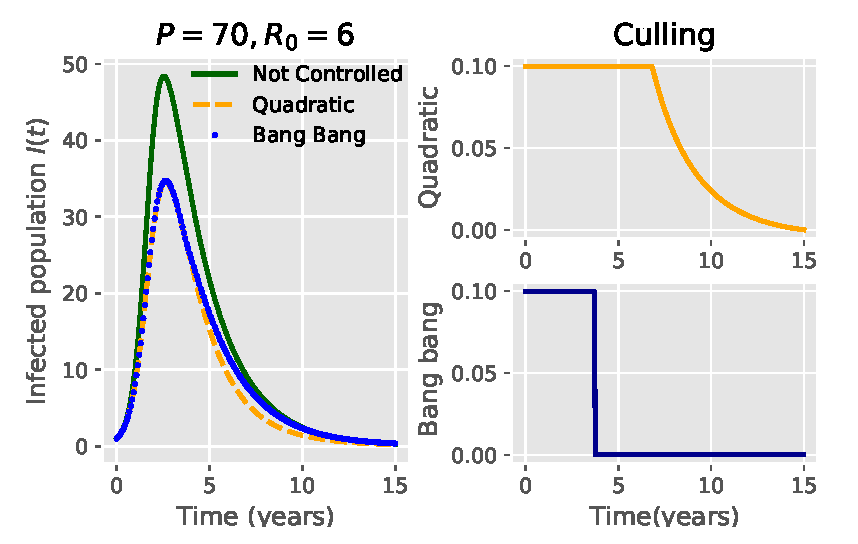
\includegraphics{Figures/figure_1_culling}
  \caption{State solutions without control, under optimal quadratic control 
  and with linear (bang-bang) control.}
  \label{fig:figure1culling}
\end{figure}

\begin{figure}[H]
  \centering
  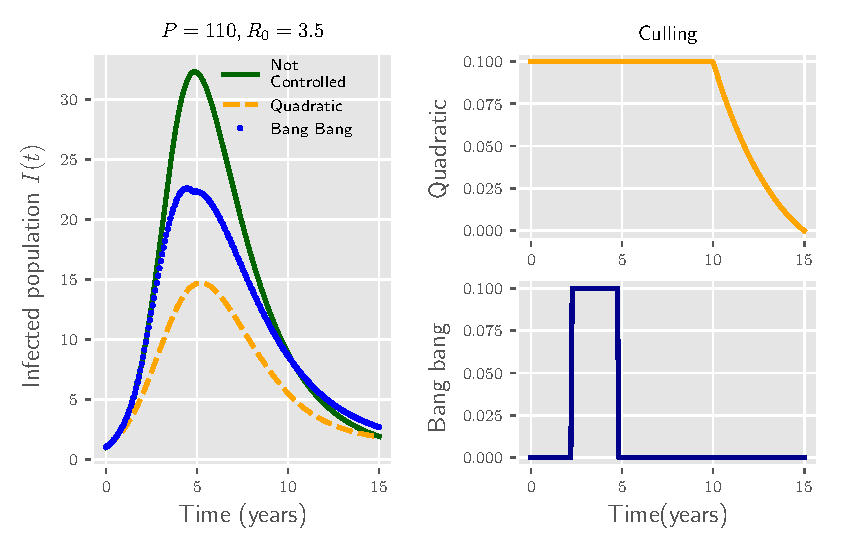
\includegraphics{Figures/figure_2_culling}
  \caption{State solutions without control, under optimal quadratic control 
  and with linear (bang-bang) control.}
  \label{fig:figure2culling}
\end{figure}

\begin{figure}[H]
  \centering
  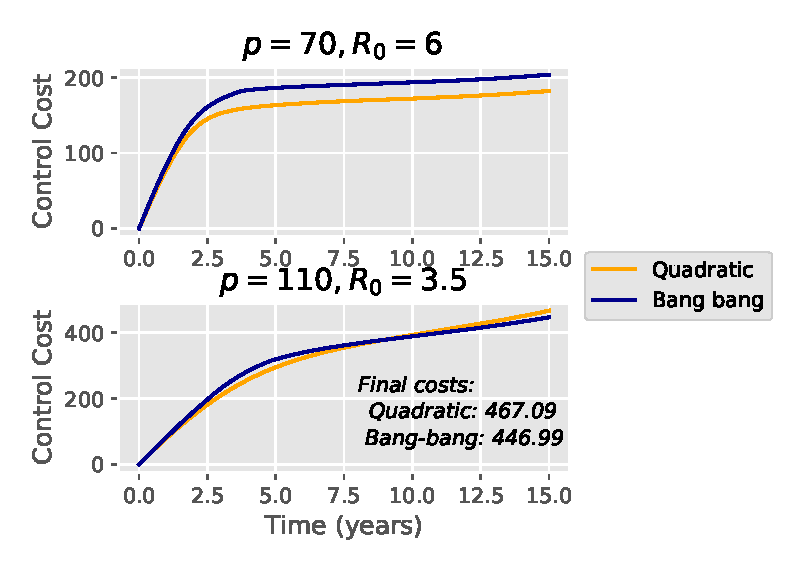
\includegraphics{Figures/figure_3_culling}
  \caption{Cost for the linear and quadratic controls under two scenes. Upper
  $P=70$, $R_0=6$, bottom, $P=110$, $R_0=3.5$, and the rest of parameters as 
  in \Cref{tbl:culling_par}.}
  \label{fig:figure3culling}
\end{figure}
    \subsection{Vaccination}
      First, we come back to the vaccination control presented in model
\eqref{eqn:epidemics_lenhart}. According to \Cref{tbl:epidemics_lenhart}
In \Cref{fig:epidemicslenhartlab7} we illustrate the effect of vaccination 
control. The simulation shows that the optimal-vaccination policy diminish
almost to zero the infected population. In color green we plot the state 
solution without control.
\begin{table}[htb]
  \begin{center}
    \begin{tabular}{rlll}
      \toprule
      \multicolumn{2}{c}{
            \textbf{Parameters values}
         }
        && \multicolumn{1}{c}{
          \textbf{Initial conditions}
        }
        \\
        \cmidrule{1-2}
        \cmidrule{4-4}
        $b$
          & \num{0.525}
          &&
          $S(0) = \num{1000}$, $E(0) = \num{100}$
        \\
        $a$, $d$ 
          & \num{0.2}, \num{0.5}
          &&
          $I(0) = \num{50}$, $R(0) = \num{15}$
        \\
        $c$
          & \num{0.0001}
        \\
        $e$
          & \num{0.5}
        \\
        $g$
          & \num{0.1}
        \\
        $A$
          & \num{0.1}
        \\
        $T$
          & \num{20.0}
        \\
      \bottomrule
    \end{tabular}
    \caption{Parameters and simulation values of the epidemic model
      \eqref{eqn:epidemics_lenhart}.}
    \label{tbl:epidemics_lenhart}
  \end{center}
\end{table}

\begin{figure}[htb!]
\centering
	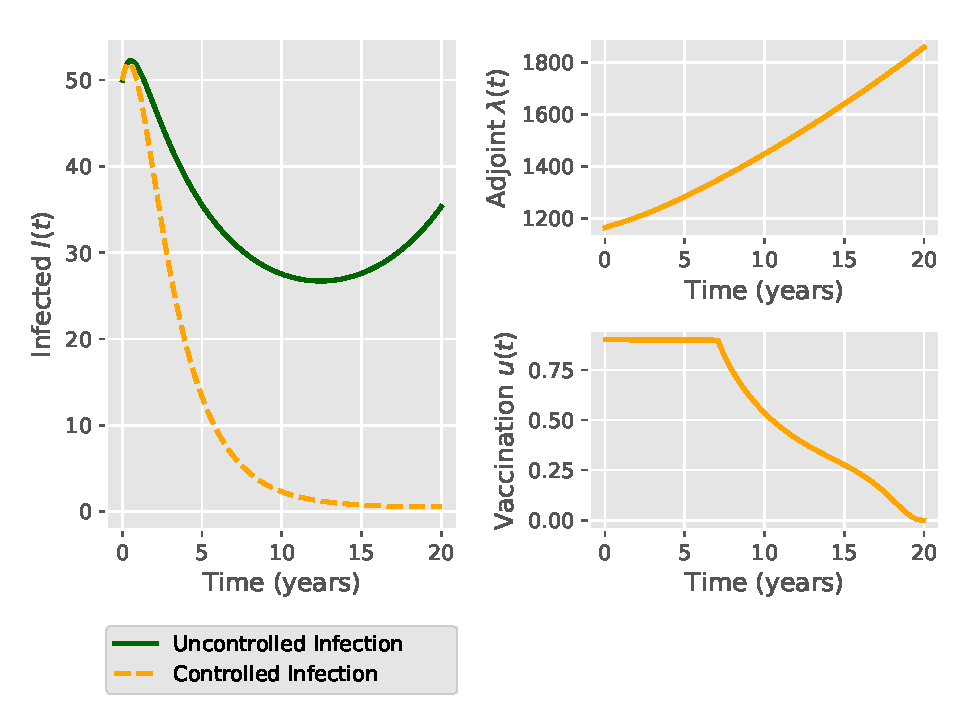
\includegraphics{./Figures/epidemics_lenhart_lab7}
	\caption{Likening between the controlled and uncontrolled Infected 
	 population.  At right, we show the optimal infected state agains the 
	 dynamics without 
	 control. At right we present the corresponding adjoint function $\lambda$ 
	 and the optimal control.}
\label{fig:epidemicslenhartlab7}
\end{figure}

    \subsection{Case finding and case control 
      in a two strain tuberculosis model}
      \begin{table}[H]
	\centering
	\begin{tabular}{rlrlll}
		\toprule
			& \multicolumn{2}{c}{
        \textbf{Parameter values}
        }
        &&&
        \multicolumn{1}{c}{\textbf{Initial Conditions}}
        \\
      \cmidrule{1-4}
      \cmidrule{6-6}
        $\beta_1$ 
            & \num{13.0}            
        &
        $\beta_2$ 
        & \num{13.0}
        &&
          $S(0) = (76/120)N$
          \\
        $\beta_3$ 
          & \num{0.0131}, 
            \num{0.0217},
        &&
        &&
          $L_1(0) = (36/120) N$
          \\
          & \num{0.029}, 
            \num{0.0436}
          &&&&
            $L_2(0) =(2/120) N$
        \\
          &&
          &&&
          $I_1(0) = (4/120)N$
        \\
        $\mu$ 
          & \num{0.0143}
          &&&&
          $I_2(0) = (1/120)N$
        \\
     	$d_1$ 
          & \num{0.0}
      &
      $d_2$ 
          & \num{0.0}
          &&
            $T(0)= (1/120)N$
     \\
     	$k_1$ 
      & \num{0.5}
      &
       $k_2$  
      & \num{1.0}
      \\
      $r_1$ 
      & \num{2.0}
      &
    $r_2$ 
      & \num{1.0}
      \\
    $p$
      & \num{0.4}
      &
      $q$
      & \num{0.1}
    \\
      $N$
      & 
        \num{6000}, 
        \num{12000}, 
      &
      $\Lambda$ 
      & $\mu N$
      \\
      &
      \num{30000}
      &&&&
      \multicolumn{1}{c}{\textbf{Control Bounds}}
      \\
      \cmidrule{6-6}
      &&&&&
        Lower \num{0.05}
      \\
      &&&&&
        Upper \num{0.95}s
      \\
      $t_f$ 
      &
        \SI{5.0}{years}
      \\
      $B_1$ 
        & \num{50.0}
      &
      $B_2$
      & \num{500.0}
      & 
      \\
      \bottomrule
    \end{tabular}
	\caption{Simulation values for the control 
	problem \eqref{eqn:MDR-TB_model}.}
	\label{tbl:parameters_MDR-TB_model}
\end{table}
%
	\Cref{fig:figure1twostraintbm} shows the effect of case finding and 
case holding controls. The combination of this strategies diminish the multi 
drug resistant population. \Cref{tbl:parameters_MDR-TB_model} compiles the 
parameters and its values used to produce this figure and fix 
$N = \num{30000}$, $\beta_3 = \num{0.29}$. To minimize the resistant TB 
population, L2 + I2, the simulation suggest that the case holding strategy 
$u_2$ would be at the upper bound during almost \SI{4.3}{years} and then 
decreasing to the lower bound. Meanwhile, decreasing value for case finding
must apply over the most of the simulated time, \SI{5}{years}. The total number 
of 
infected resistant TB $L2 + I2$  at the final time $t_f = \SI{5}{years}$ results
\num{1123}. This same number but without control sums 4176. So this policies 
prevents \SI{3053}{cases} of resistant TB.

  According with \Cref{tbl:parameters_MDR-TB_model} and taking different values
for the parameter $\beta_3$, in \Cref{fig:figure2twostraintbm} we illustrate 
the effect of parameter $\beta_3$ over controls.The 
simulation suggest that both controls experiment small variations just at the 
beginning and reach almost the same level after \SI{5}{year}. As wee see the 
simulation suggest that just delay the same profile for few months.
%
\begin{figure}[H]
  \centering
  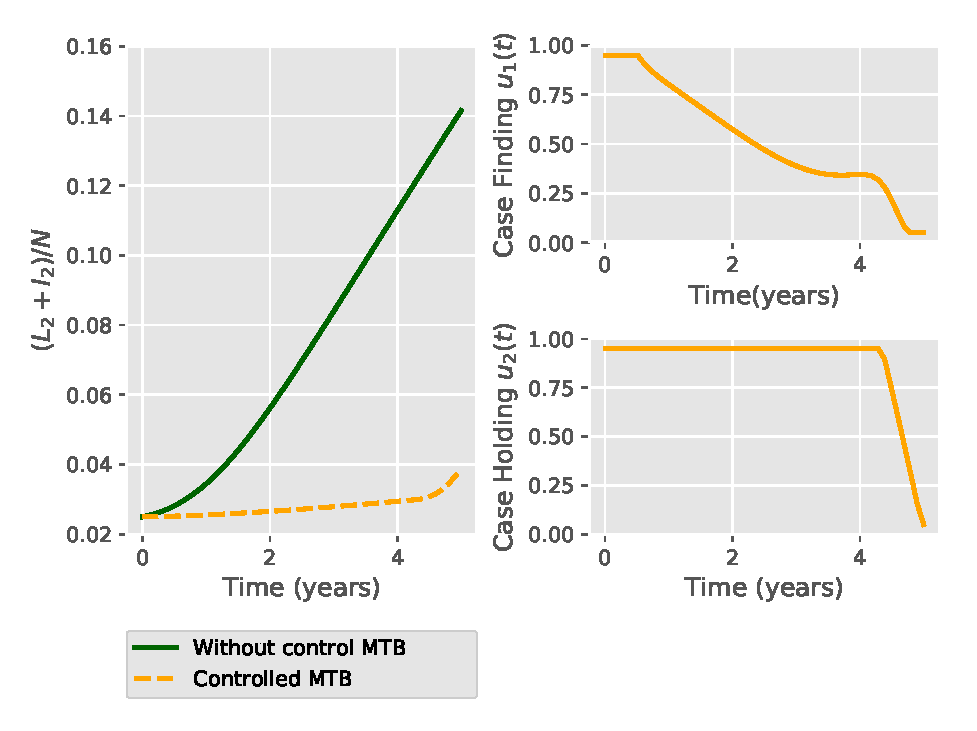
\includegraphics{Figures/figure_1_two_strain_tbm}
  \caption{Normalized infected population according to parameters of 
  \Cref{tbl:parameters_MDR-TB_model}. Here the green line represents the 
  infected population without control. As we see, combining case finding 
  $u_1(t)$ and  case holding $u_2(t)$, dramatically diminish the density of 
  infected with resistant TB.}
  \label{fig:figure1twostraintbm}
\end{figure}

%
\begin{figure}[H]
  \centering
  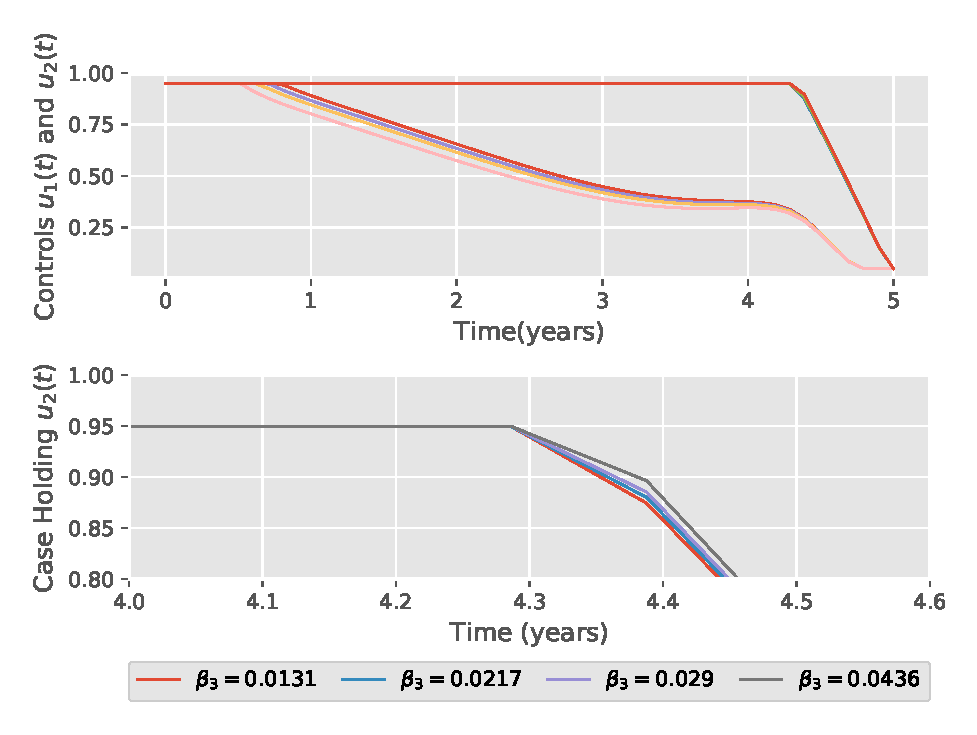
\includegraphics{Figures/figure_2_two_strain_tbm}
  \caption{
    Top case finding and case holding controls 
    under parameters encased in \Cref{tbl:parameters_MDR-TB_model} and
    different values of parameter $\beta_3$. At bottom we capture a smaller
    region to illustrate the variations regarding to case holding. Simulation 
    suggest 
    that case holding remains almost with the same profile, while case finding 
    delays same period for only for a few months.
  }\label{fig:figure2twostraintbm}
\end{figure}

\Cref{fig:figure3twostraintbm} illustrates case finding and case holding 
strategies under population of different sizes. The simulation suggest that
under relative small population, is more important holds case finding at the 
top. While for relatively bigger population the case holding is the more 
important strategy.
\begin{figure}[H]
  \centering
  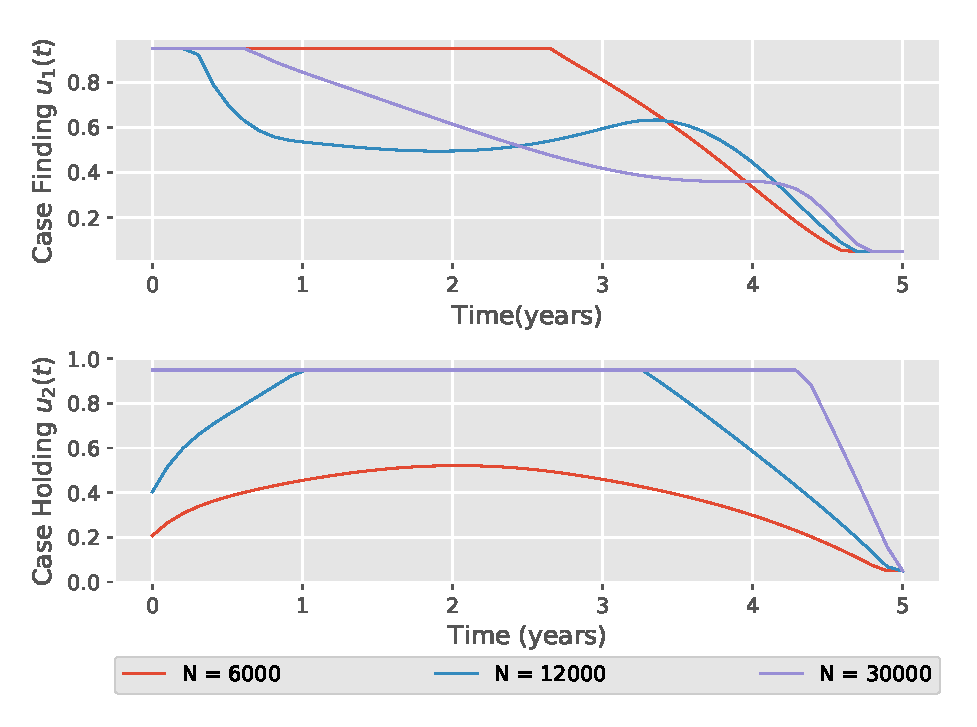
\includegraphics{Figures/figure_3_two_strain_tbm}
  \caption{
    The effect of different size of populations. For 
    relatively small population, the case finding strategy is more important 
    than case finding, meanwhile for  bigger populations, the case holding 
    plays a more important role. The rest of parameters as in 
    \Cref{tbl:parameters_MDR-TB_model}.
  }
  \label{fig:figure3twostraintbm}
\end{figure}

    \subsection{Isolation and quarantine for SARS} 
      \subsection*{SARS}
\begin{table}[H]
    \begin{center}
      \begin{tabular}{@{}rlrl@{}}
        \toprule
        \multicolumn{4}{c}{\bf{Parameters values}}
        \\
        \midrule
        $\beta$
          & \num{0.2}
          & $d_1$, $d_2$
          & \num{0.0079}, \num{0.0337}
        \\
        $\varepsilon_E$, 
        $\varepsilon_Q$,
        $\varepsilon_J$
          & \num{0.3}, \num{0.0}, \num{0.1}
          &
          $k_1$, $k_2$ 
          & 
            \num{0.1},
            \num{0.125}
          \\
        $\mu$
          & \num{0.000034}
        \\
        $\Lambda$
          & $\mu N$
        \\
        $p$
          & \num{0.0}
        \\
        $\sigma_1$, $\sigma_2$
          & \num{0.0337}, \num{0.0386}
          && \multicolumn{1}{c}{\bf{Initial conditions}}
        \\
        \cmidrule{4-4}
          &&& $S(0)=\num{12e6}$, $E(0)=1565$,
         \\
        $t_f$
          & $\SI{1.0}{year}$
          && $Q(0)=292$, $I(0)=\num{695}$,
        \\
        Step size
        & $dt=\SI{1.0}{day}$
        && $J(0)=\num{326}$, $R(0)=\num{20}$
        \\
        $u_i$ bounds
          & \num{.05}, \num{0.5}
        \\
        $B_1$, $B_2$, $B_3$, $B_4$
        & \num{1.0}, \num{1.0}, \num{1.0}, \num{1.0}
        \\
        $C_1$, $C_2$
        & \num{300}, \num{600}
        \\
        \bottomrule
      \end{tabular}
     \caption{Parameter description for the SARS model
     \eqref{eqn:sars_model}.}
     \label{tbl:sars_table}
     \end{center}
\end{table}

\begin{figure}[H]
  \centering
  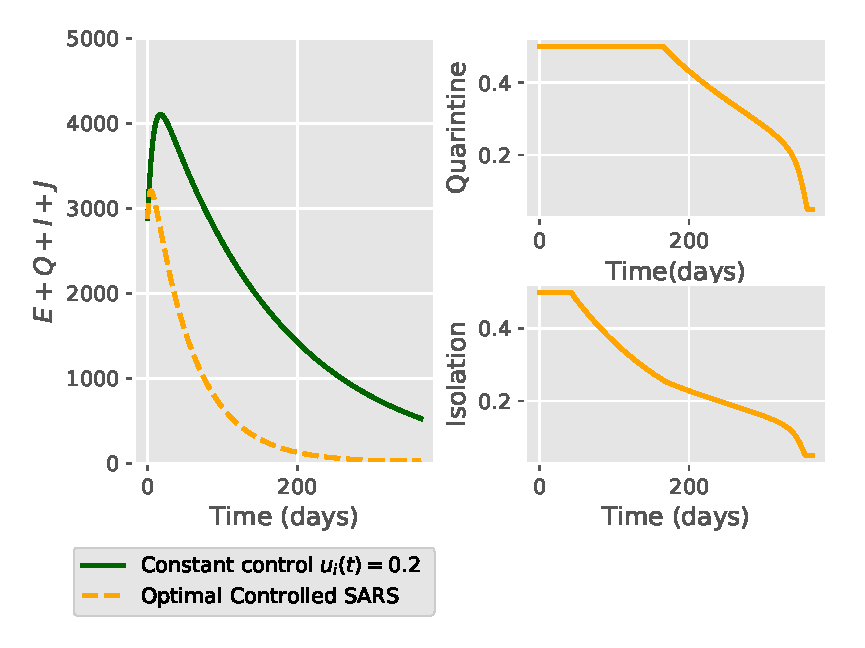
\includegraphics{Figures/figure_1_sars}
  \caption{At left, a likening of the whole infected population
  without constant control and under the optimal policy. }
  \label{fig:figure1sars}
\end{figure}

\begin{figure}[H]
  \centering
  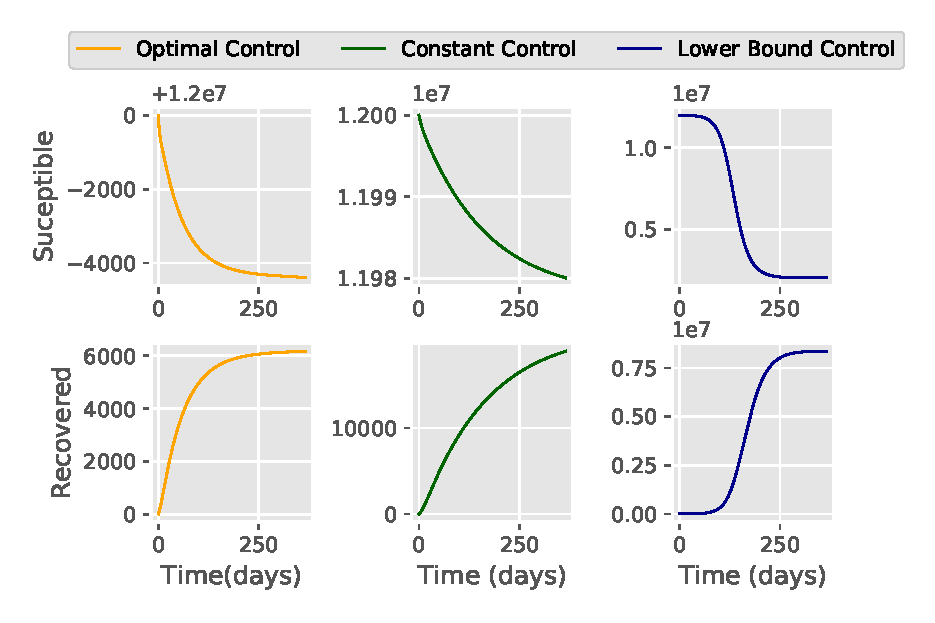
\includegraphics{Figures/figure_2_sars}
  \caption{Susceptible and recover populations under
  optimal, constant and lower bound policies.}
  \label{fig:figure2sars}
\end{figure}

\begin{figure}[H]
  \centering
  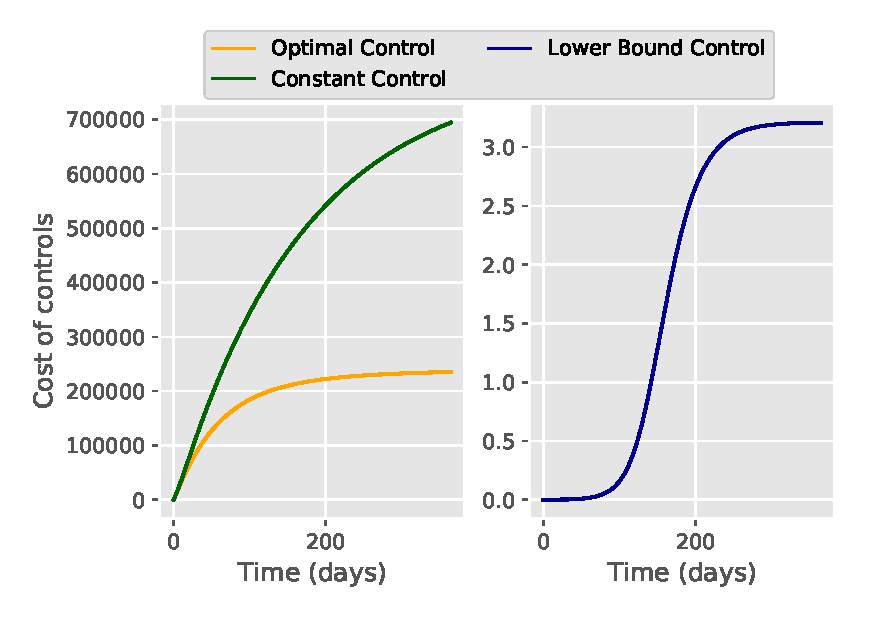
\includegraphics{Figures/figure_3_sars}
  \caption{
    Cost of control-disease for the optimal, constant and lower bound
    policies, see \Cref{eqn:sars_cost}.
  }
  \label{fig:figure3sars}
\end{figure}
%
  \section{Concluding remarks}
   \paragraph{\it Uniqueness of optimal policy}
The proof of the uniqueness of the state path $X_u$, given a policy $u$, is
fairly standard (Theorem \ref{ExAdmisPair}). However, the uniqueness of an 
{\it optimal policy} is not trivial and it can be established on some small 
enough interval; see, for instance, \cite{GaffSchaefer09} and the references 
therein.  
\medskip

\paragraph{\it Maximum principle vs. Dynamic programming} 
  The same approach is followed in almost all the related literature on optimal
control of epidemics/diseases. As an alternative, the so-called Dynamic
programming approach can be used to analyze this kind of problems. With the
Maximum principle we need to solve a system of ordinary differential equations
(ODEs) whereas in Dynamic programming a partial differential equation (PDE)
arises. In addition, both approaches involve an optimization problem. The
Maximum principle is mostly used because there are plenty of methods to
numerically solve ODEs.
\medskip
\paragraph{\it Numerical Issues}

\medskip
\paragraph{\it Evolutionary algorithms}
Evolutionary algorithms are a kind of heuristics algorithms well 
suited for global optimization. Such algorithms emulate natural
evolution introducing operators for mutation ($\mathbf{M}$), crossover 
($\mathbf{C}$) and selection ($\mathbf{S}$). One of the earliest works
on evolutionary methods was developed by George E. P. Box \cite{Box1957}.
Nevertheless, it can be said tat the first evolutionary algorithm at
least as they are known today, was the so called Genetic Algorithm (GA) 
introduced by J. H. Holland \cite{JHH1975}. Since then many variations of
evolutionary algorithms have been developed being Differential Evolution (DE),
introduced by Price and Storn \cite{Storn1997}, one of the simplest yet efficient and 
effective optimization algorithms. Algorithm \ref{alg:DE1} shows the 
general form of Evolutionary Algorithms for optimizing the $fob$ 
objective function. There, an initial population $Y$ of size $N_p$, 
generated in the search space $\mathcal{V}$ by the operator $\mathbf{Y}_0$;
is subject to the evolutionary process until certain stopping criterion is 
met. Then the best individual ($\mathbf{y}_{best}$), i.e., the individual who
optimizes $fob$, is selected by introducing the operator $\mathbf{Best}$. 
In Algorithm \ref{alg:DE1} the variable $M$ stores a mutated population, 
the variable $C$ stores the results of the crossover operator. The selection
operator selects from $M$ and $C$ the individuals which will conform the new
population $Y$. This selection is based in some criteria usually dictated by the
objective function. For instance, if $\mathbf{y}$ is an element of $Y$
and $\mathbf{c}$ an element of $C$, a common criterion for minimization is 
to select $\mathbf{y}$ if $fob(\mathbf{y})<fob(\mathbf{c})$.
A detailed explanation for constructing the main operators 
$\mathbf{M}$, $\mathbf{C}$ and $\mathbf{S}$, can be found in
\cite{Bagchi1999} for GA and in \cite{Price_Storn2005} for the DE
algorithm.
%
\begin{algorithm}[H]
\caption{Evolutionary Algorithms}
\label{alg:DE1}
\begin{algorithmic}
% \small
\State $Y$ $\leftarrow$ $\mathbf{Y}_0(Np,\mathcal{V})$
\While{(the stopping criterion has not been met)}
\State $M$ $\leftarrow$  $\mathbf{M}(Y)$
\State $C$ $\leftarrow$  $\mathbf{C}(Y,C)$
\State $Y$ $\leftarrow$  $\mathbf{S}(Y,C,fob)$ 
\EndWhile
\State $\mathbf{y}_{best} \leftarrow \mathbf{Best}(Y, fob)$
\end{algorithmic}
\end{algorithm}%


Regarding the optimal control policies problem, the evolutionary 
method is commonly applied by using piecewise constant functions for the 
controllers $u_k$, $k=1,2,\dots,n$. For instance, the optimization of a
quantity of the form
\begin{equation}
J(u_1,u_2,\dots,u_n) = \int_0^T{\left[ \mathcal{L}(t) + w_1\,u_1^2(t) + 
w_2\,u_2^2(t)+\dots + w_n\,u_n^2(t) \right]\,dt},
\label{eq:Jaccion}
\end{equation}
with weight constants $w_k$, can be conducted by discretizing the 
interval $I = [0,T]$ {\color{red}(cerrado o abierto, ustedes decidan)} in disjoints subintervals $I_j$ and choosing  
\begin{equation}\label{DECrossover}
u_{k}(t) =
\begin{cases}
u^j_{k} & \text{if $t \in I_j$}
\vspace*{0.1cm}\\
0 & \text{otherwise.}
\end{cases}
\end{equation}
Usually the functional under the sign of integral in Eq. (\ref{eq:Jaccion})
obeys certain dynamical model which need to be solved but in such a way
that $J$ be optimized. Now, the numbers $u^j_{k}$ will be part of an 
individual who will be subject to the evolutionary process. This approach 
has been followed for example in \cite{Yan2008} and \cite{Jang2018}, 
respectively for the GA and the DE algorithms. {\color{red} Nevertheless,
it would be quite
interesting to address the problem of considering the control functions 
as  general differentiable functions (or at least combinations of a 
small subset of some well known functions and operators) in the whole 
interval $I$ (or almost everywhere in I, or except in a finite number of 
points in $I$). As far as we know, there is no work addressing the optimal control policies problem in this manner, and thus this paragraph intends to motivate further research in this direction.} (no se si poner esto ultimo que puse en rojo, arreglen la redaccion segun convenga)


  \section{Appendix: Deterministic OCPs in continuous time}
    \subsection{Deterministic OCPs in continuous time}

Let $\mathbf{X}\s\R^n$ and $\mathbf{U}\s \R^m$ be nonempty sets. The sets $\mathbf{X}$ and $\mathbf{U}$ are 
respectively called the {\it state space} and the {\it control space}. Consider 
the following {\it control system}
\begin{equation}\label{CoDiffEq}
\dot{X}(t)=f(t,X(t),u(t)),\qquad t\in[0,T], \quad X(0)=x_0.
\end{equation}
where $f:[0,T]\times \mathbf{X}\times \mathbf{U}\to \R^n$ and $u:[0,T]\to U$. 
%In order to guarantee the existence of a solution $x$ to \eqref{CoDiffEq}, 
%we need the following.

\begin{assumption}\label{Assum1}  The function $f:[0,T]\times \mathbf{X}\times \mathbf{U}\to \R^n$
is measurable and there exists a constant $L>0$ such that
\begin{eqnarray}
  \|f(t,x,u)-f(t,x_1,u)\| & \leq & L\|x-x_1\|\label{LipfInx}\\
  \|f(t,0,u)\| & \leq & L\label{fBound}
\end{eqnarray}
for every $x,x_1\in \mathbf{X}$, $t\in[0,T]$, and $u\in \mathbf{U}$.
\end{assumption}

%A proof of the following result can be found, for instance, in Yong \cite[Sect. 2.1]{Yong2015}. 

\begin{theorem}\label{ExAdmisPair} 
	Under Assumption \ref{Assum1}, for each measurable function 
	$u:[0,T]\to \mathbf{U}$, there exists a unique absolutely continuous function $X_u$ that satisfies the the system 
	\eqref{CoDiffEq} almost everywhere. %The solution $x_u$ satisfies	\begin{equation}\label{ineqSol} 
	%	|x_u(t)|\leq e^{Lt}(1+|x_0|) -1,\qquad t\in [0,T].	\end{equation}
\end{theorem}
\begin{proof} Let $u:[0,T]\to U$ be a measurable function. Consider the linear space 
    \[\mathbb{X}=\{X:[0,T]\to \R^n\mid X \mbox{ is continuous}\}\] 
with the norm
    \[ \|X\|_w:=\sup_{t\in[0,T]} \frac{|X(t)|}{w(t)}, \]
where $w(t):=e^{Lt}$ for each $t\in [0,T]$. It can be shown, with slight modifications in \cite[Section 2.1]{Teschl}, that the pair $(\mathbb{X},\|\cdot\|_w)$ is a Banach space. Define the operator $K:\mathbb{X}\to \mathbb{X}$ by 
    \[ K[X](t):=x_0 + \int_0^t f(s,X(s),u(s))ds.\]
By \eqref{LipfInx} and \eqref{fBound}, any $(t,x,u)$ satisfies 
  \begin{equation}
      \|f(t,x,u)\| \leq  L(1+\|x\|),
  \end{equation}
thus $f(\cdot,X(\cdot),u(\cdot))$ is Lebesgue integrable and $K[X]$ is absolutely continuous. We claim that $K$ is a contraction with contraction constant $1-e^{-LT}$. Indeed,
    \begin{eqnarray*}
    \| K[X] - K[Y] \|_w & = & \sup_{t\in[0,T]} \frac{|\int_0^t [f(s,X(s),u(s)) -f(s,Y(s),u(s))]ds|}{w(t)}\\
        & \leq &   \sup_{t\in[0,T]} \frac{L\int_0^t w(s)[w(s)]^{-1}|X(s) -Y(s)|ds}{w(t)}\\
        &\leq &  L\|X-Y\|_w \sup_{t\in[0,T]} \frac{\int_0^t w(s)ds}{w(t)}\\
        & = &  L\|X-Y\|_w \sup_{t\in[0,T]}\frac{[e^{Lt}-1]/L}{e^{Lt}}\\
        & = &  (1-e^{-LT})\|X-Y\|_w. 
    \end{eqnarray*}
Then by Banach's fixed point theorem \cite[Theorem 2.1]{Teschl}, there exists a unique $X\in \mathbb{X}$ satisfying 
    \[ X(t)=x_0 + \int_0^t f(s,X(s),u(s))ds.\]
Therefore \eqref{CoDiffEq} holds almost everywhere \cite[Corollary 5.4.1]{Loeb2016}.
\end{proof}


	Given a measurable function $u$ and the solution $X_u(\cdot)$ to 
\eqref{CoDiffEq}, the terminal state $X_u(T)$ can be constrained to belong to a set $M\s X$, in such a case we assume the following. 

\begin{assumption} Let $M$ be a nonempty subset of $\mathbf{X}$. 
	The set of {\it admissible controls} 
	\begin{equation}\label{FeasCont}  
		 \mathbb{U}_M:=\{u:[0,T]\to \mathbf{U}\mid u\  
		 \mbox{\rm is measurable and } X_u(T)\in M\} 
	\end{equation}
	is nonempty. A pair $(u,X_u)$, where $u\in \mathbb{U}_M$, is called an 
	{\it admissible pair}. To ease notation, we simply write $(u,X)$.
\end{assumption}


Consider the {\it performance index} or {\it cost functional} of an admissible control $u$, given the initial state $x_0$, 
        \begin{equation}\label{PiBolza} V(u,x_0) := \int_0^Tg(t,X(t),u(t))\,dt + h(X(T)),\end{equation}
where $g:[0,T]\times \mathbf{X}\times \mathbf{U}\to \R$ and $h:\mathbf{X}\to\R$ are measurable.

The {\it optimal control problem} (OCP) consists of finding an admissible control $u^\ast$ such that
\[ V(u^\ast,x_0)=\sup\{ V(u,x_0)\mid u\in \mathbb{U}_M \}.\]
If there exists such a control $u^\ast$, then it is called an {\it optimal policy} or {\it optimal control}. The pair $(X^\ast,u^\ast)$, where $X^\ast$ is given by Theorem \ref{ExAdmisPair}, is called an {\it optimal pair}.



\begin{remark}\rm
The performance index \eqref{PiBolza} is said to be in the {\it Bolza form}. When $g= 0$ and $h\neq 0$, it is said to be in the {\it Mayer form}. Another form occurs when $h= 0$ and $g\neq 0$; in such a case, \eqref{PiBolza} is said to be in the {\it Lagrange form}. These three forms are equivalent; see, for instance, Cesari \cite[Sect. 1.9]{Cesari83}. 
\end{remark} 

%%------------------------------------------------------------------------------

\subsection{Existence of optimal policies}




\begin{assumption}
The functions $g$ and $h$ in the performance index \eqref{PiBolza}
 
\end{assumption}










%%------------------------------------------------------------------------------
\subsection{The maximum principle}


The following lemma is a classical result in Calculus of Variations. We give a proof for completness.

\begin{lemma}\label{VariatLemma} Let  

\end{lemma}




%%------------------------------------------------------------------------------
\subsection{Sufficient conditions}







%
  \bibliographystyle{plainnat}
  \bibliography{references,OptimalControl-ContinuousControledEpidemicModels}
\end{document}